Here we present the model reported in \cite*{Bolzoni2014} to describe a 
outbreak of bovine tuberculosis. The regarding uncontrolled model reads

\begin{equation}
	\begin{aligned}
  \min_{u(t)\in \mathcal{U}}
    &
    \int_0^T
      I(t) + P [u(t)]^{\theta}, \quad \theta \in \{1,2\},
      \quad P = B/A
  \\ \textrm{subject to:} &
  \\
    &\dfrac{dS}{dt} =
			\underbrace{
			r S 
			\left (
				1 - \dfrac{S+I}{K}
			\right)
			}_{:=G(S,I)}
			 - \beta SI - u(t) S
		\\
		&\dfrac{dI}{dt} =
			\beta SI - (\alpha + \mu + u(t)) I.
	\end{aligned}
\end{equation}
%
\begin{figure}[h]
  \centering
  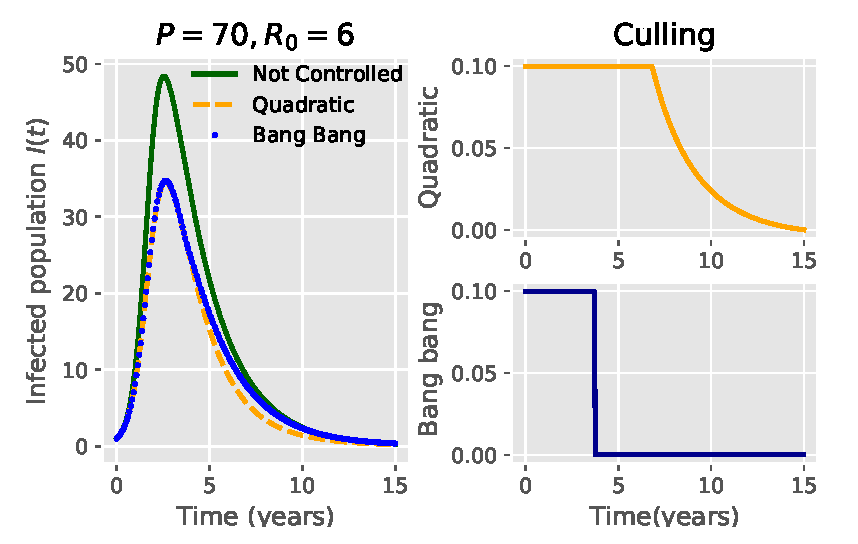
\includegraphics{Figures/figure_1_culling}
  \caption{State solutions without control, under optimal quadratic control 
  and with linear (bang-bang) control.}
  \label{fig:figure1culling}
\end{figure}

\begin{figure}[h]
  \centering
  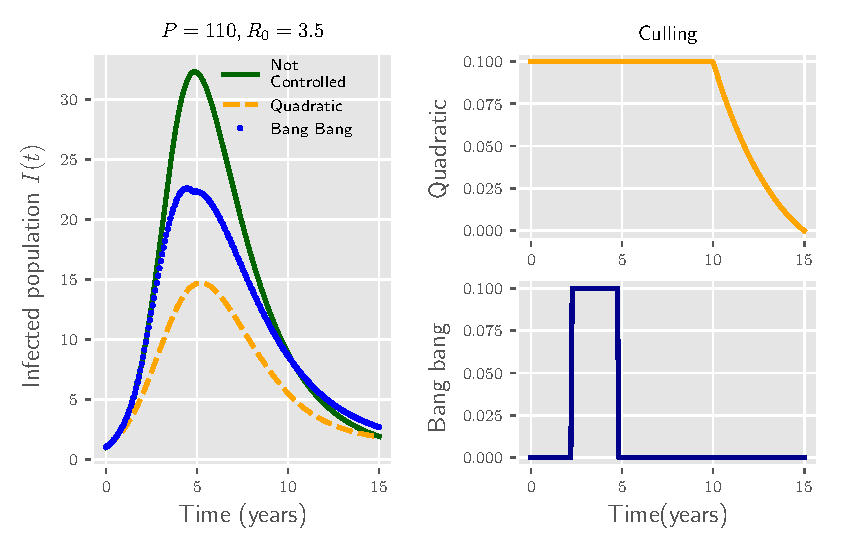
\includegraphics{Figures/figure_2_culling}
  \caption{State solutions without control, under optimal quadratic control 
  and with linear (bang-bang) control.}
  \label{fig:figure1culling}
\end{figure}

\begin{figure}[h]
  \centering
  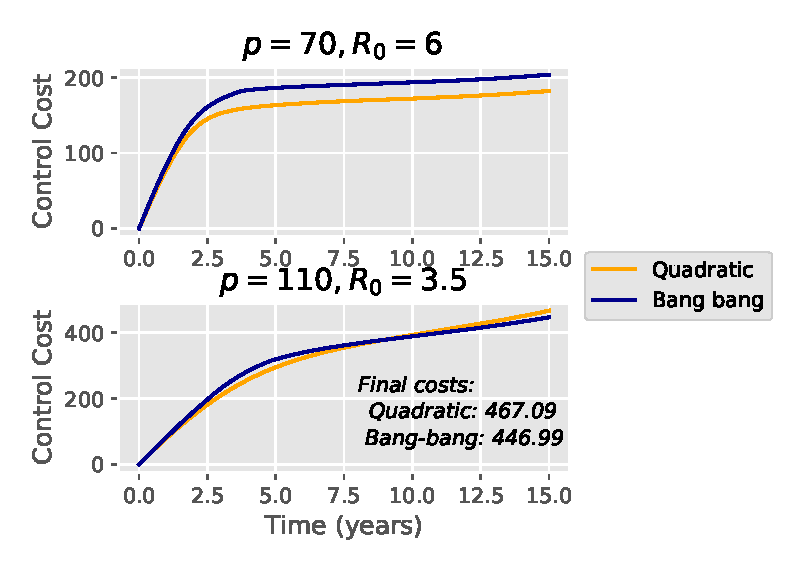
\includegraphics{Figures/figure_3_culling}
  \caption{Cost for the linear and quadratic controls under two scenes. Upper
  $P=70$, $R_0=6$, bottom, $P=110$, $R_0=3.5$, and the rest of parameters as 
  in table}
  \label{fig:figure1culling}
\end{figure}